\section{GEM}
Contact person: Andy White (awhite@uta.edu)
\subsection{Introduction}
The High Energy Physics group at UTA has been developing a new type of calorimetry, based on the Particle Flow technique, for experiments at the future International Linear Collider. White proposed the application of GEM~\cite{Sauli1997531} technology to digital hadron calorimetry. Basic requirements include, the ability to achieve a high level of transverse and longitudinal segmentation, a MIP signal well separated from the noise level, a high density front-end readout to handle the large number of channels, and flexibility in the design and implementation of a variety of active layer sizes in realistic size modules. GEM technology offers a viable and attractive solution to these requirements.
\begin{figure}
	\centering
	\begin{minipage}{.495\textwidth}
		\centering
	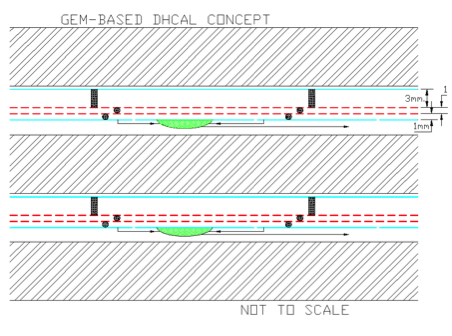
\includegraphics[width=\textwidth]{Calorimeter/GEM_HCAL/crossSection}
	\caption{Concept for a Digital Hadron GEM-based Calorimeter}
	\label{fig:Calorimeter:GEM:crossSection}
	\end{minipage}\hfill
	\begin{minipage}{.495\textwidth}
		\centering
	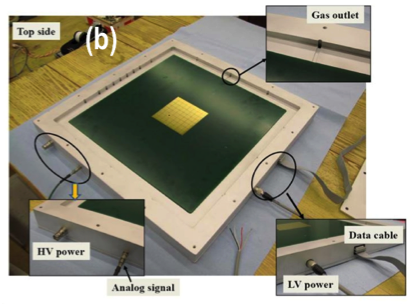
\includegraphics[width=\textwidth]{Calorimeter/GEM_HCAL/prototype}
	\caption{Concept for a Digital Hadron GEM-based Calorimeter}
	\label{fig:Calorimeter:GEM:prototype}
	\end{minipage}
\end{figure}
\begin{figure}
	\centering
	\begin{minipage}{.33\textwidth}
		\centering
		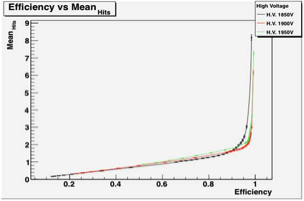
\includegraphics[width=\textwidth]{Calorimeter/GEM_HCAL/multiplicityVSefficiency}
		\caption{Hit multiplicity vs. efficiency}
		\label{fig:Calorimeter:GEM:multiplicityVSefficiency}
	\end{minipage}\hfill
	\begin{minipage}{.33\textwidth}
		\centering
		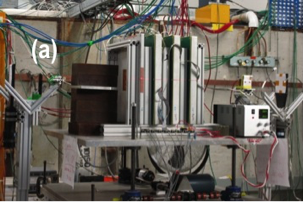
\includegraphics[width=\textwidth]{Calorimeter/GEM_HCAL/chamberStack}
		\caption{GEM chamber stack}
		\label{fig:Calorimeter:GEM:chamberStack}
	\end{minipage}\hfill
	\begin{minipage}{.33\textwidth}
		\centering
		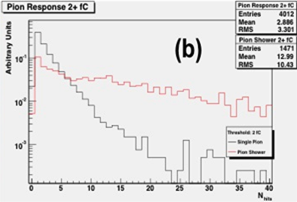
\includegraphics[width=\textwidth]{Calorimeter/GEM_HCAL/pionBeam}
		\caption{Pion beam (single/showers)}
		\label{fig:Calorimeter:GEM:pionBeam}
	\end{minipage}
\end{figure}
Our proposed digital hadron calorimeter (Figure~\ref{fig:Calorimeter:GEM:crossSection}) comprises a stack of steel absorbers, of sufficient thickness to contain hadronic showers, interlaced with active gaseous sampling-elements.

\subsection{Recent Milestones}
A series of prototype detectors (Figure~\ref{fig:Calorimeter:GEM:prototype}) has already been constructed and tested using $\unit[10]{cm} \times \unit[10]{cm}$ GEM foils from CERN and $\unit[30]{cm} \times \unit[30]{cm}$ GEM foils from 3M Corporation and CERN~\cite{1742-6596-404-1-012031}. The KPiX chip from SLAC was used for the readout. KPiX has a four-deep pipeline, on-board DAC charge injection calibration, and a Wilkinson 13-bit ADC for each of its 1024 channels. Results from exposure to cosmic rays, and an external, scintillator trigger, yielded MIP detection efficiency of 95\%, in agreement with simulation predictions. The corresponding hit multiplicity, the average number of hits seen in a single active layer when one particle passes through, was measured to be 1.7 (Figure~\ref{fig:Calorimeter:GEM:multiplicityVSefficiency}).
This predicts only little confusion in track following and energy cluster definition in a final calorimeter system. A gas mixture of Argon 80\%, \ce{CO2} 20\% was used throughout these initial studies, and for which a most probable signal size of \unit[10]{fC} was measured for a MIP. The detector gain was about 3,500. Various chambers (Figure~\ref{fig:Calorimeter:GEM:chamberStack}) were also exposed to a test beam at Fermilab, with satisfactory stable performance for single pions (non-interacting) and showers induced by steel absorber in front of the chambers~\cite{White:GEM:SiDWS2015}.
\subsection{Engineering Challenges}
\begin{figure}
	\centering
	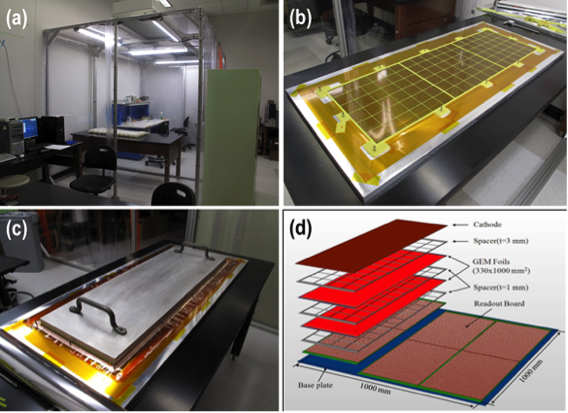
\includegraphics[width=.5\textwidth]{Calorimeter/GEM_HCAL/activitySummary}
	\caption{Large scale GEM chamber activity at UTA: (a) Purpose-built clean room for handling large foils,
(b) partially assembled $\unit[33]{cm} \times \unit[100]{cm}$ double-GEM chamber, (c) glue curing stage under pressure plate,
(d) schematic view of three $\unit[33]{cm} \times \unit[100]{cm}$ chambers integrated in a $\unit[1]{m^2}$ chamber.}
	\label{fig:Calorimeter:GEM:activitySummary}
\end{figure}
CERN has demonstrated that large area GEM foils can be successfully produced using the single-side etching technique. This technology would need to be available from a commercial manufacturer for large quantity production. The main challenges would then be the assembly of many different size double-GEM chambers, for the 40 layers of a DHCAL, the longitudinal division of the barrel chambers, with solutions to the provision of high voltage and gas through multiple chambers and the extraction/readout of the signals from the large number of small pads.
\subsection{Future Plans}
The next stage in the development of GEM-based DHCAL is the construction of large area chambers. We have received and qualified five $\unit[33]{cm}\times\unit[100]{cm}$ large GEM foils. We are developing the mechanical structure, the electronic readout board schemes and the schemes for integrating the three unit chambers ($\unit[33]{cm}\times\unit[100]{cm}$) into one $\unit[1]{m}\times\unit[1]{m}$ plane (Figure~\ref{fig:Calorimeter:GEM:activitySummary}). We plan to construct and test two of these $\unit[33]{cm}\times\unit[100]{cm}$ unit chambers initially.
Work on the large chambers is currently waiting the resumption of support for ILC detector activities in the U.S.
